\subsubsection{Template method} % (fold)
\label{ssub:template_method}

Definisce lo scheletro di un algoritmo, delegando alcuni dei passi a
sottoclassi. Permette alle sottoclassi di ridefinire alcuni passi di un
algoritmo senza cambiarne la struttura.

\begin{figure}[h!]
  \centering
  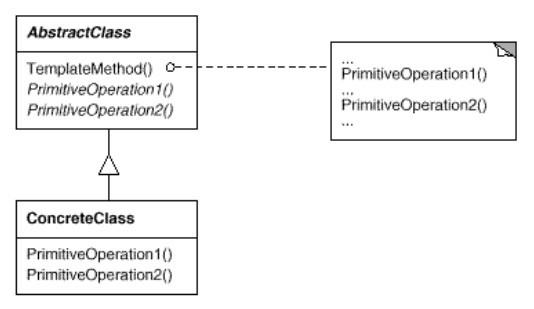
\includegraphics[scale=0.5]{imgs/template-method}
  \caption{Diagramma delle classi del pattern `Template method'}
\end{figure}

Il pattern si può applicare nei seguenti casi:

\begin{itemize}
  \item Quando vogliono implementare una sola volta le parti invarianti di un
  algoritmo, lasciando la ridefinizione delle parti variabili alle sottoclassi;
  \item Quando si vuole fattorizzare un comportamento comune tra diverse
  sottoclassi per evitare duplicazione.
\end{itemize}
